% Figure 3.2 (Session 3): the two solvable limits of the spinless chain.
% The image is rendered by figures/blender/s3_2_cdw_limits.py; the coordinates of the labels
% come from figures/blender/out/cdw_limits_anchors.tex. Compile with:
%   pdflatex cdw_limits.tex ; result moves to ../many_body_fermions/cdw_limits.pdf
\documentclass[11pt,tikz,border=0pt]{standalone}
\usepackage{amsmath,amssymb,graphicx}
\usepackage{xcolor}
\definecolor{coursedark}{HTML}{1B2A4A}
\definecolor{costamber}{HTML}{B8620A}
\newlength{\figw}\setlength{\figw}{16.19cm}   % the text width of the notes (letter, 2.7 cm margins), so labels print at size

\begin{document}
\begin{tikzpicture}[lbl/.style={font=\small, text=coursedark}]
  \node[anchor=south west, inner sep=0pt] at (0,0)
    {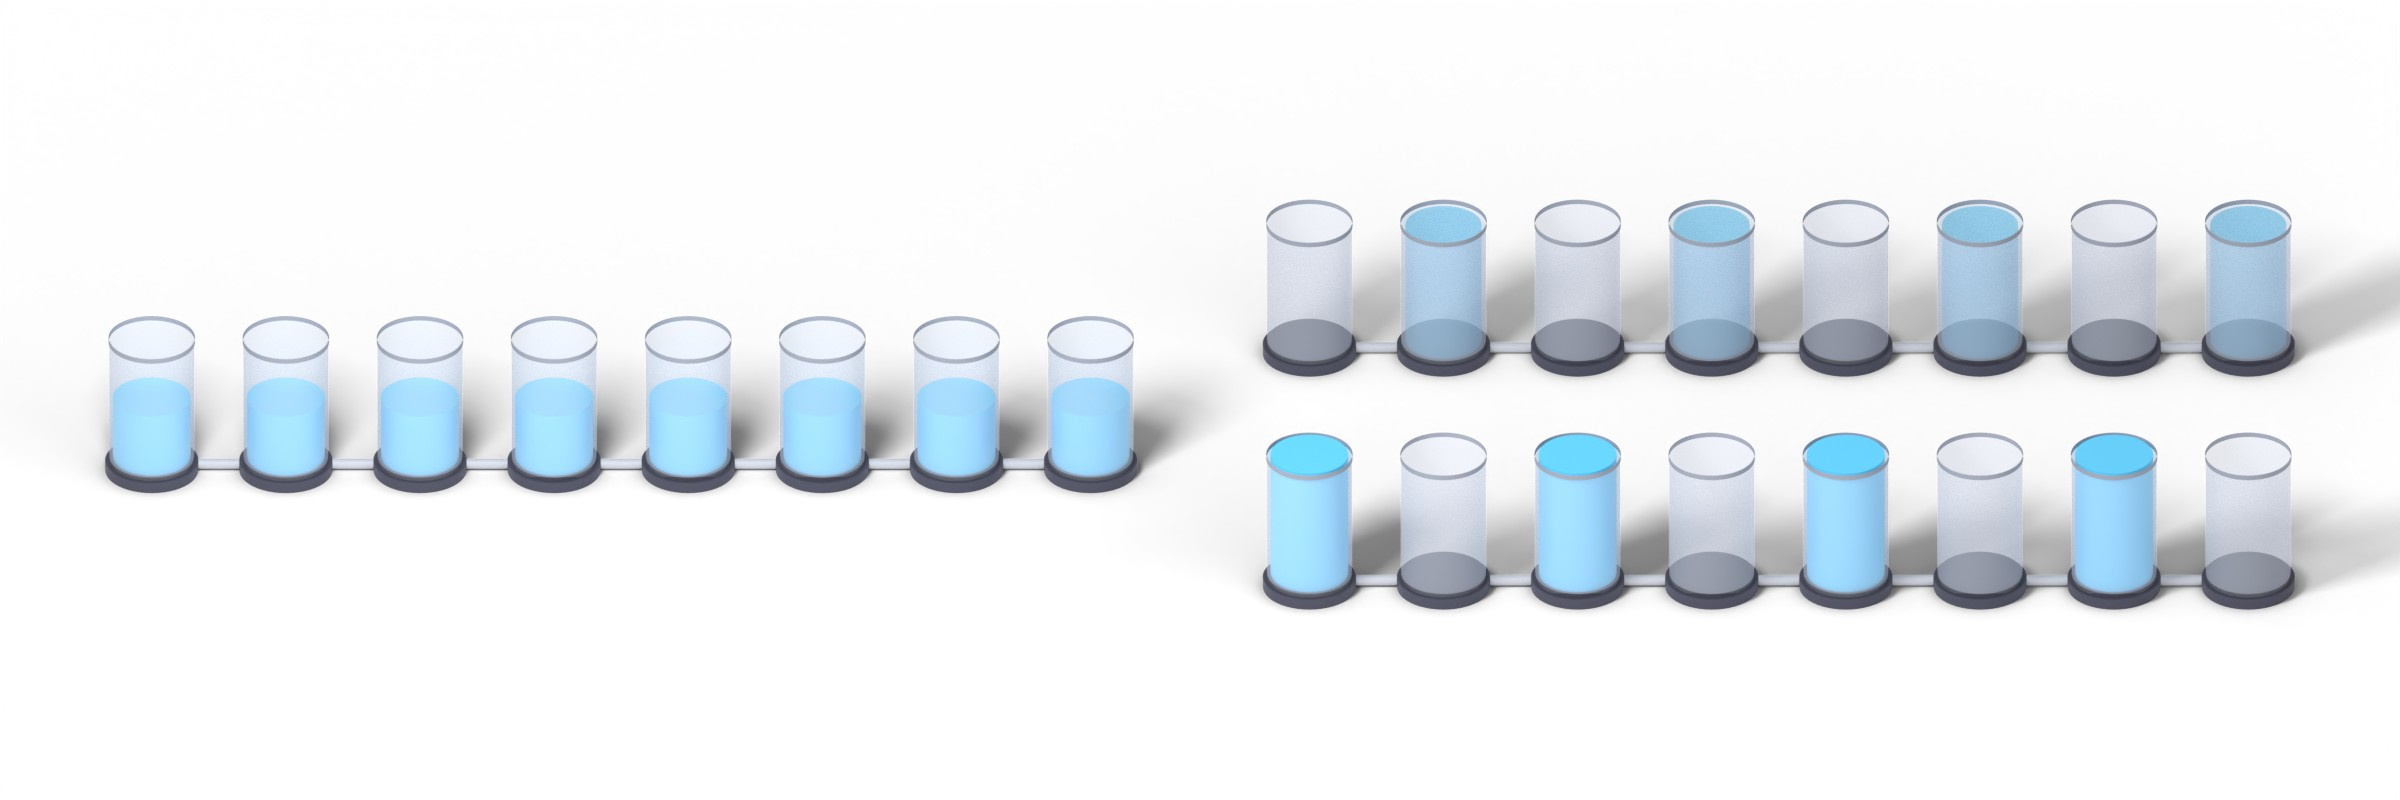
\includegraphics[width=\figw]{../blender/out/cdw_limits.jpg}};
  %% written by figlib.py; x and y in units of the image width
\coordinate (a) at (0.0118\figw,0.3033\figw);
\coordinate (nA) at (0.2588\figw,0.1170\figw);
\coordinate (b) at (0.4941\figw,0.3033\figw);
\coordinate (front) at (0.7412\figw,0.0685\figw);
\coordinate (back) at (0.7412\figw,0.2523\figw);

  \node[lbl, font=\normalsize, anchor=west] at (a) {(a)\quad$V=0$};
  \node[lbl, font=\normalsize, anchor=west] at (b) {(b)\quad$V\to\infty$};
  \node[lbl, anchor=north] at (nA) {$\langle n_i\rangle=\tfrac12$ on every site, one ground state};
  \node[lbl, anchor=north] at (front) {$1,0,1,0,\dots$};
  \node[lbl, anchor=south] at (back) {its partner, shifted by one site, same energy};
\end{tikzpicture}
\end{document}
